\chapter{Needs, Requirements, \& Specifications}
\label{needs-and-specs}
The project needs encapsulate specific components of the project that the final prototype must accomplish in order to be successful. The needs table was developed from the initial project statement provided by our client and was further iterated on after subsequent meetings with him and the team’s research. 
An important need that was identified was the safety of the team. After the main development of the final prototype it was found that dropping the vehicle into free-fall from a height of 10 m contained risks that we did not have the infrastructure to mitigate. Some of these risks include failure of rotor deployment, failure to control the motion of the vehicle, fracturing of components and subsequent ballistic fragment motion, and the destruction of the vehicle. Instead of performing the functions of the prototype all together with a drop test, the team focused on a safer alternative that would aim at testing each individual mechanism within a controlled environment. Figures \ref{needs-table} and \ref{needs-limits-table} show the needs that the team identified and the metrics that are used to test the functionality of the design.

\begin{figure}
    \centering
    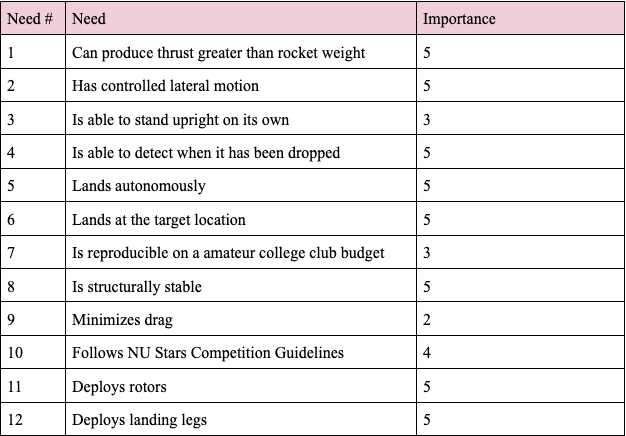
\includegraphics[width=1.0\textwidth]{src/figs/needstable.png}
    \caption{Design Needs \\ *Importance ranked on a scale from 1-5, where 5 is the highest}
    \label{needs-table}
\end{figure}


\begin{figure}
    \centering
    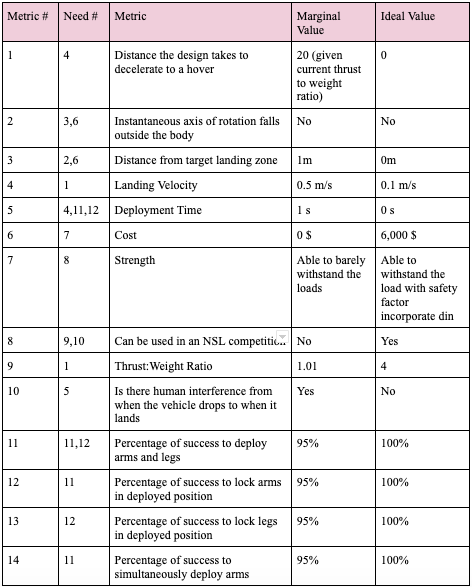
\includegraphics[width=1.0\textwidth]{src/figs/metricstable.png}
    \caption{Acceptable Limits for Metrics}
    \label{needs-limits-table}
\end{figure}